\documentclass[aspectratio=169]{../latex_main/tntbeamer}  % you can pass all options of the beamer class, e.g., 'handout' or 'aspectratio=43'
\usepackage{dsfont}
\usepackage{bm}
\usepackage[english]{babel}
\usepackage[T1]{fontenc}
%\usepackage[utf8]{inputenc}
\usepackage{graphicx}
\graphicspath{ {./figures/} }
\usepackage{algorithm}
\usepackage[ruled,vlined,algo2e,linesnumbered]{algorithm2e}
\usepackage{hyperref}
\usepackage{booktabs}
\usepackage{mathtools}

\usepackage{amsmath,amssymb}

\DeclareMathOperator*{\argmax}{arg\,max}
\DeclareMathOperator*{\argmin}{arg\,min}

\usepackage{amsbsy}
\newcommand{\vect}[1]{\bm{#1}}
%\newcommand{\vect}[1]{\boldsymbol{#1}}

\usepackage{pgfplots}
\pgfplotsset{compat=1.16}
\usepackage{tikz}
\usetikzlibrary{trees} 
\usetikzlibrary{shapes.geometric}
\usetikzlibrary{positioning,shapes,shadows,arrows,calc,mindmap}
\usetikzlibrary{positioning,fadings,through}
\usetikzlibrary{decorations.pathreplacing}
\usetikzlibrary{intersections}
\pgfdeclarelayer{background}
\pgfdeclarelayer{foreground}
\pgfsetlayers{background,main,foreground}
\tikzstyle{activity}=[rectangle, draw=black, rounded corners, text centered, text width=8em]
\tikzstyle{data}=[rectangle, draw=black, text centered, text width=8em]
\tikzstyle{myarrow}=[->, thick, draw=black]

% Define the layers to draw the diagram
\pgfdeclarelayer{background}
\pgfdeclarelayer{foreground}
\pgfsetlayers{background,main,foreground}

% Requires XeLaTeX or LuaLaTeX
%\usepackage{unicode-math}

\usepackage{fontspec}
%\setsansfont{Arial}
\setsansfont{RotisSansSerifStd}[ 
Path=../latex_main/fonts/,
Extension = .otf,
UprightFont = *-Regular,  % or *-Light
BoldFont = *-ExtraBold,  % or *-Bold
ItalicFont = *-Italic
]
\setmonofont{Cascadia Mono}[
Scale=0.8
]

\renewcommand{\ttdefault}{Cascadia Mono}

% scale factor adapted; mathrm font added (Benjamin Spitschan @TNT, 2021-06-01)
%\setmathfont[Scale=1.05]{Libertinus Math}
%\setmathrm[Scale=1.05]{Libertinus Math}

% other available math fonts are (not exhaustive)
% Latin Modern Math
% XITS Math
% Libertinus Math
% Asana Math
% Fira Math
% TeX Gyre Pagella Math
% TeX Gyre Bonum Math
% TeX Gyre Schola Math
% TeX Gyre Termes Math

% Literature References
\newcommand{\lit}[2]{\href{#2}{\footnotesize\color{black!60}[#1]}}

%%% Beamer Customization
%----------------------------------------------------------------------
% (Don't) Show sections in frame header. Options: 'sections', 'sections light', empty
\setbeamertemplate{headline}{empty}

% Add header logo for normal frames
\setheaderimage{
	% 
\includegraphics[height=\logoheight]{figures/TNT_darkv4.pdf}
	
\includegraphics[height=\logoheight]{../latex_main/figures/Leibniz-AI-Academy_Logo}
	% 
\includegraphics[height=\logoheight]{figures/logo_tntluh.pdf}
}

% Header logo for title page
\settitleheaderimage{
	% 
\includegraphics[height=\logoheight]{figures/TNT_darkv4.pdf}
	
\includegraphics[height=\logoheight]{../latex_main/figures/Leibniz-AI-Academy_Logo}
	% 
\includegraphics[height=\logoheight]{figures/logo_tntluh.pdf}
}

% Title page: tntdefault 
\setbeamertemplate{title page}[tntdefault]  % or luhstyle
% Add optional title image here
%\addtitlepageimagedefault{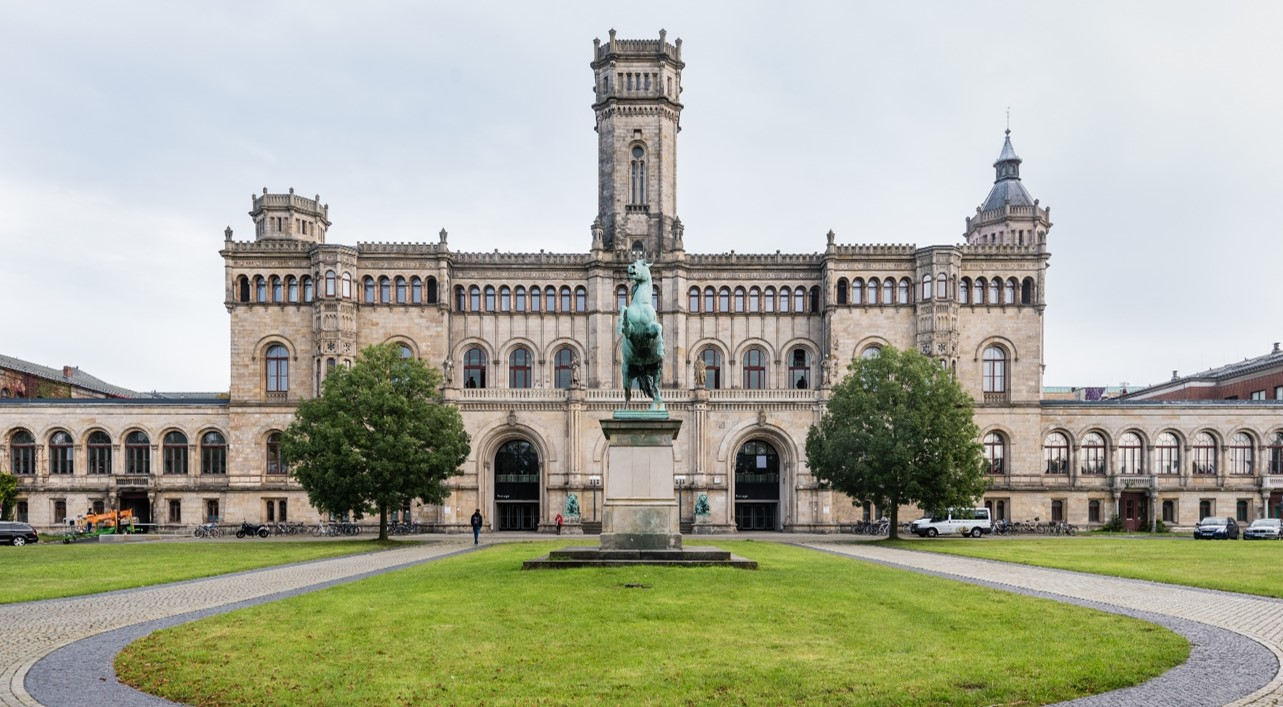
\includegraphics[width=0.65\textwidth]{figures/luh_default_presentation_title_image.jpg}}

% Title page: luhstyle
% \setbeamertemplate{title page}[luhstyle]
% % Add optional title image here
% \addtitlepageimage{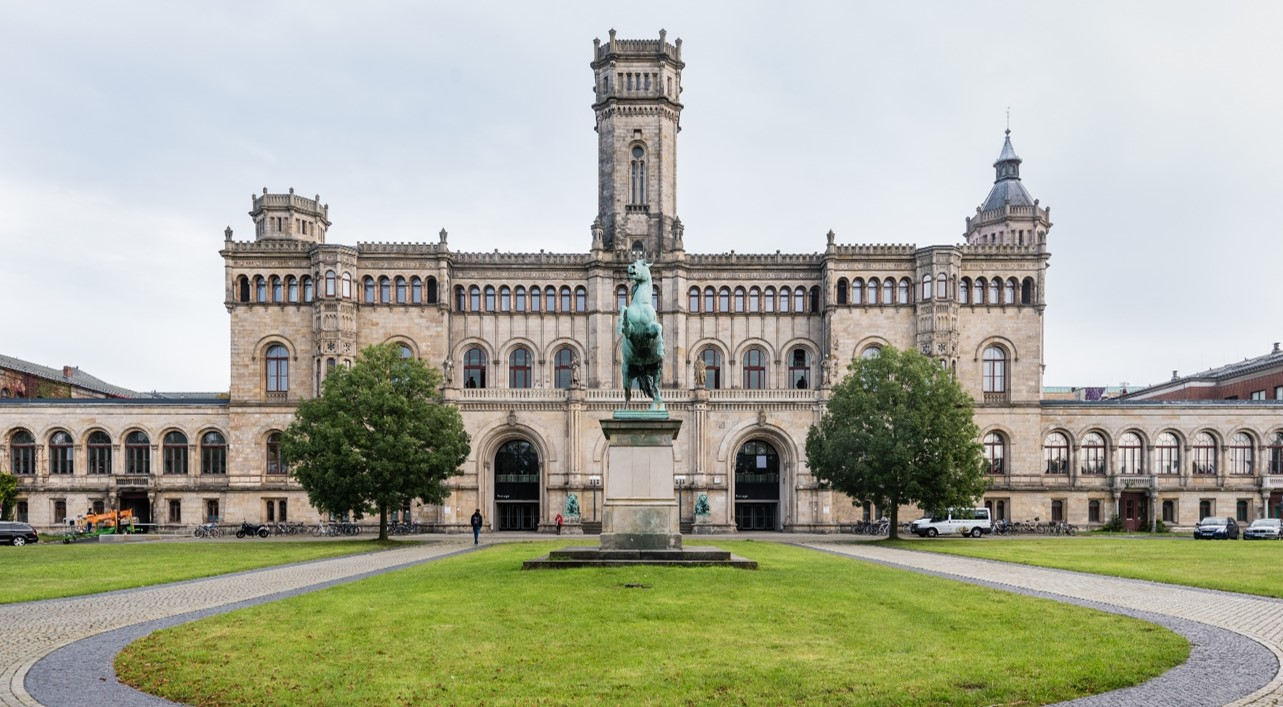
\includegraphics[width=0.75\textwidth]{figures/luh_default_presentation_title_image.jpg}}

\author[Abedjan \& Lindauer]{Ziawasch Abedjan \& \underline{Marius Lindauer}\\[1em]
	%
\includegraphics[height=\logoheight]{../latex_main/figures/luh_logo_rgb_0_80_155.pdf}\qquad
	
\includegraphics[height=\logoheight]{../latex_main/figures/DBIS_Kurzlogo.png}\qquad
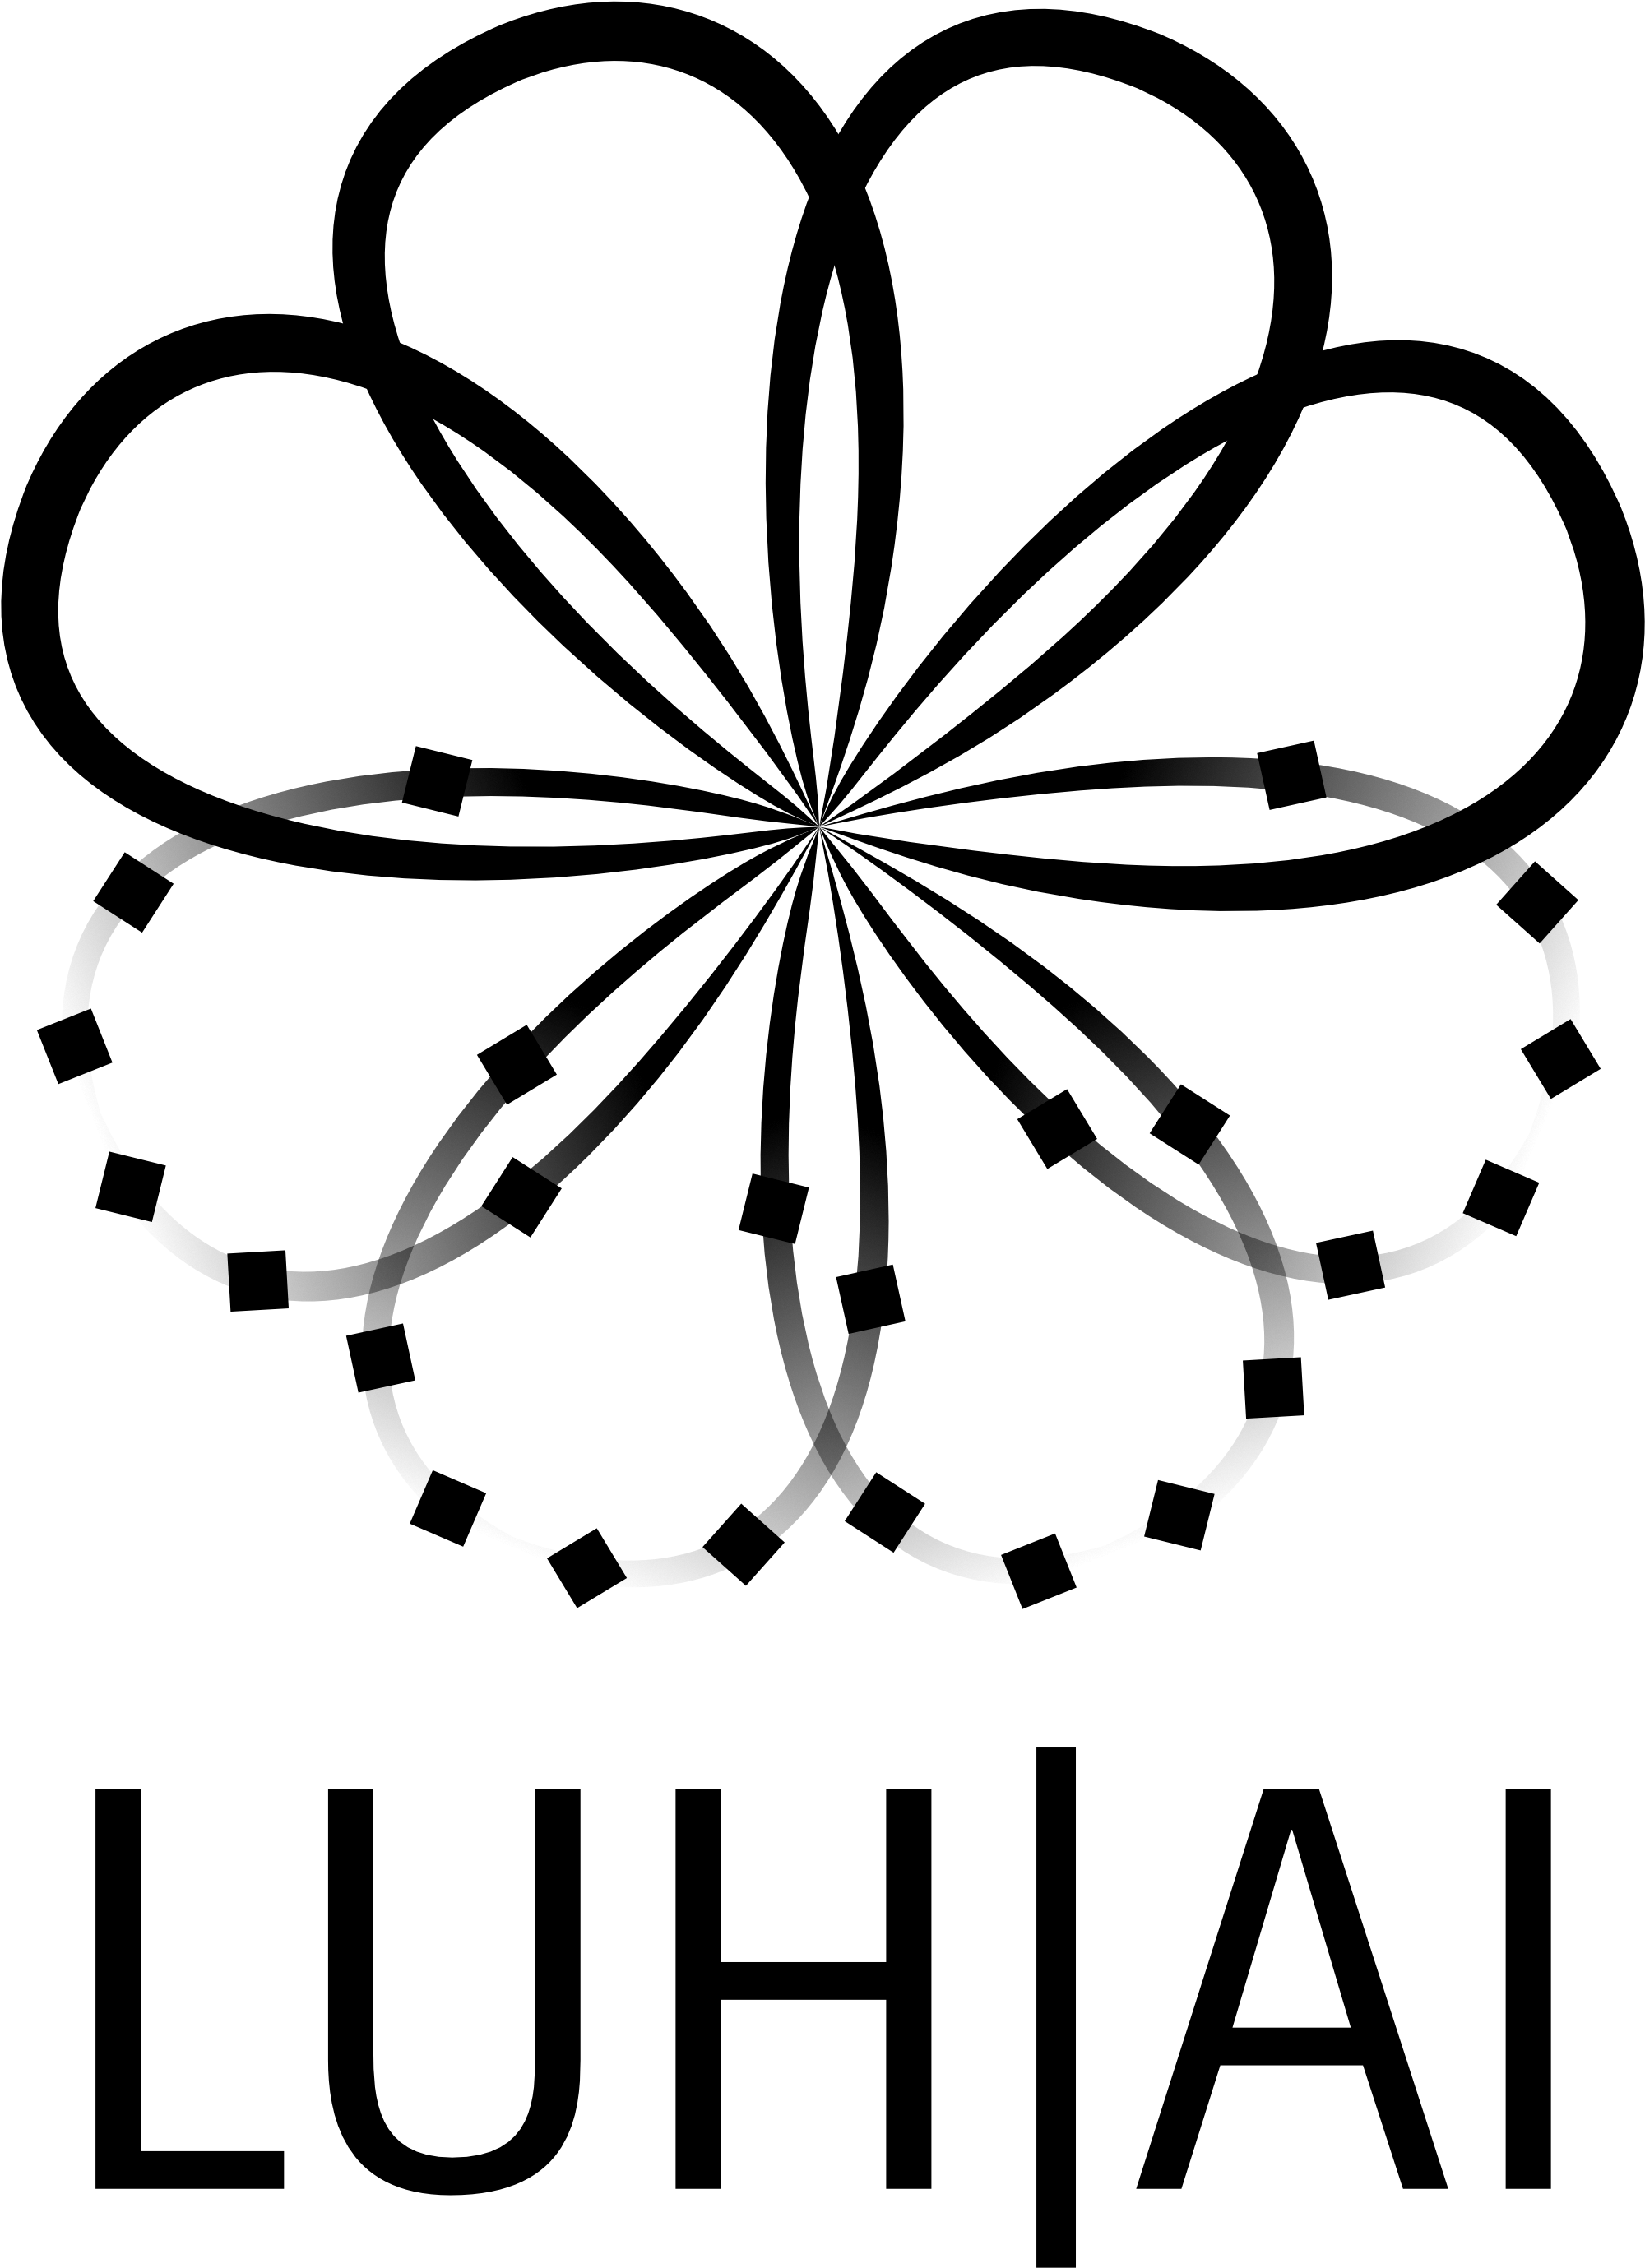
\includegraphics[height=\logoheight]{../latex_main/figures/logo_short_highres_black}\qquad

\includegraphics[height=\logoheight]{../latex_main/figures/Leibniz-AI-Academy_Logo}\qquad
%
\includegraphics[height=\logoheight]{../latex_main/figures/L3S.jpg}	
}
\date{\hspace{0.5em} {
\includegraphics[height=1.5em]{../latex_main/figures/Cc-by-nc-sa_icon.svg.png}}; extension of \href{https://ds100.org/fa21/}{[DS100]}
}


%%% Custom Packages
%----------------------------------------------------------------------
% Create dummy content
\usepackage{blindtext}

% Adds a frame with the current page layout. Just call \layout inside of a frame.
\usepackage{layout}


%%% Macros
%\renewcommand{\vec}[1]{\mathbf{#1}}
% \usepackage{bm}
%\let\vecb\bm

\title[Statistics]{DS: Data Sampling and Probability}
\subtitle{Statistics}

\graphicspath{ {./figure/} }
%\institute{}


\begin{document}
	
	\maketitle
	

% Slide 54: Empirics
\begin{frame}{Empirics}
    \begin{itemize}
        \item In science, the word “empirical” means “observed”.
        \begin{itemize}
            \item Observed birds in the sky
            \item Observed car crashes at a round-about
        \end{itemize}
        \item Empirical distributions are distributions of observed data, such as data in random samples.
    \end{itemize}
\end{frame}

% Slide 55: Inference
\begin{frame}{Inference}
    \textbf{Statistical Inference:}
    \begin{itemize}
        \item Making conclusions based on data in random samples        
        \item Example:\\
        \textbf{Task}: Use the data to guess the value of an unknown (fixed) number.\\
        \textbf{Approach}: Create an estimate of the unknown quantity!\\
        \textbf{Remark}: Depends on the random samples.
    \end{itemize}
\end{frame}

% Slide 56: What is a statistic?
\begin{frame}{What is a statistic?}
    \begin{itemize}
        \item A single piece of data.
        \item A numerical summary of a dataset 
        \begin{itemize}
            \item function of realizations of RVs
            \item Often the \textbf{expected value}
        \end{itemize}
        
    \end{itemize}
    \textbf{What is an estimator?} \\
    A statistic designed to estimate a parameter.
\end{frame}
	
 
 \begin{frame}{Statistic / Estimator}
	    \begin{columns}
	        \begin{column}{.4\textwidth}

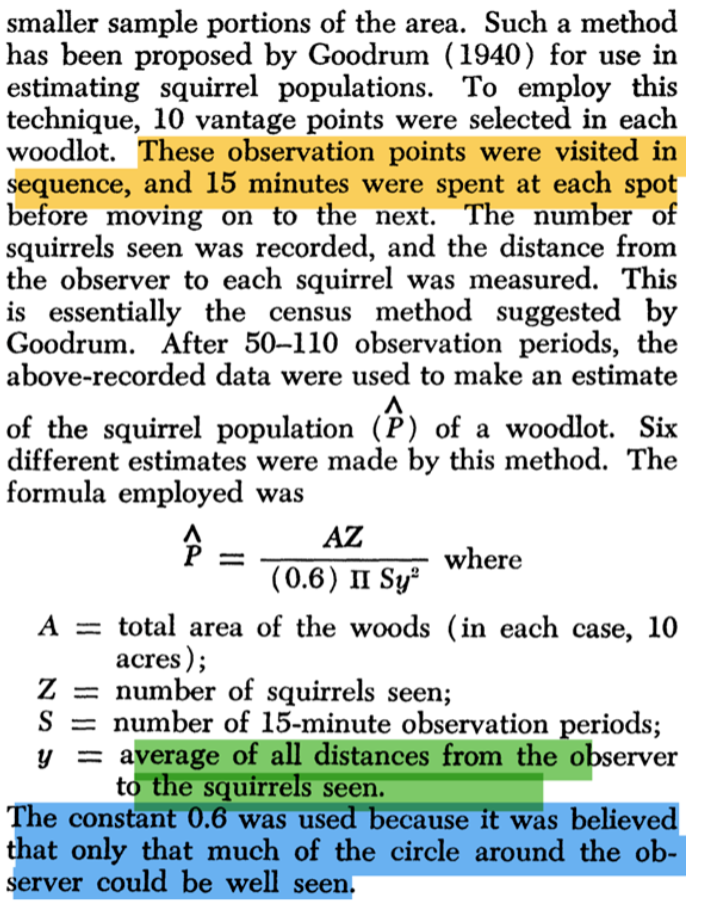
\includegraphics[scale=.38]{figure/squirrel_stat}
	       
	        \end{column}
	            
	        \begin{column}{.4\textwidth}
	            
	            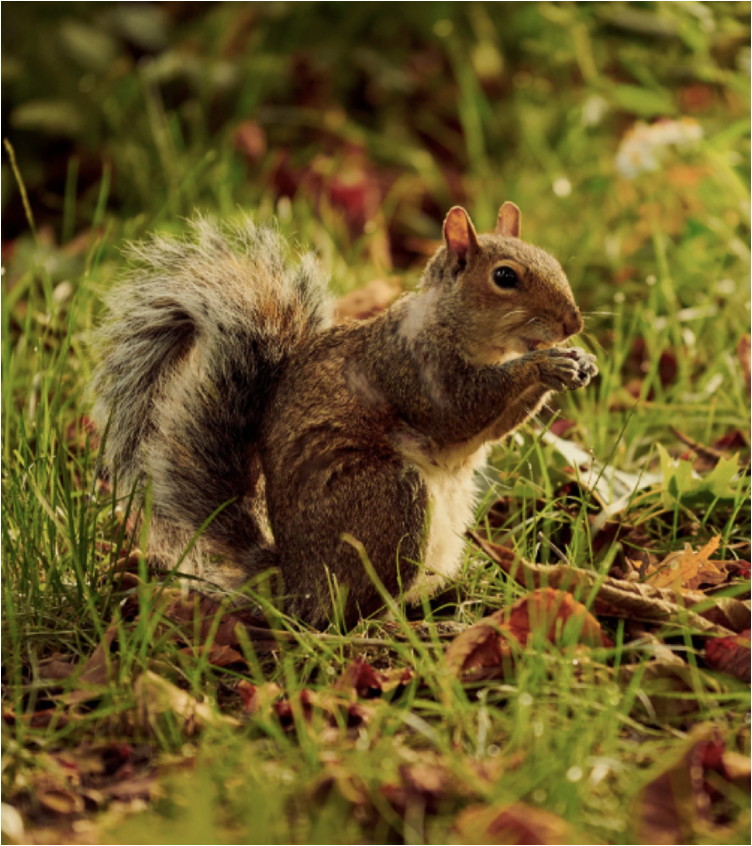
\includegraphics[scale=.45]{Bild2}
	            
	        \end{column}
	        
	        \end{columns}
	\end{frame}

% Slide 58: Expected Value
\begin{frame}{Expected Value}
    The \textbf{expected value} of a random variable $X$ is the weighted average of the values of $X$, where the weights are the probabilities of the values.

    \begin{itemize}
        \item Expected value is a number, not a random variable.
        \item It is analogous to the average.
            \begin{itemize}
                \item It has the same units as the random variable.
                \item It doesn’t need to be a possible value of the random variable.
                \item It is the center of gravity of the probability histogram.
            \end{itemize}
    \end{itemize}

$$\mathbb{E}(X) = \sum_{\text{all } x_i } x_i P(X=x_i) = \mu$$
    
\end{frame}

% Slide 59: Properties of Expectations
\begin{frame}{Properties of Expectations}
    \textbf{Linear transformations:}\\
    Let $a$ and $b$ be constants. Then,
    \begin{equation}
        \mathbb{E}(aX + b) = a\mathbb{E}(X) + b
    \end{equation}

    \textbf{Additivity:}\\
    Let $X$ and $Y$ be independent random variables. Then,
    \begin{equation}
        \mathbb{E}(X + Y) = \mathbb{E}(X) + \mathbb{E}(Y)
    \end{equation}

    \textbf{Linearity of Expectation:}\\
    Let $X_1, X_2, \dots, X_n$ be random variables. Then,
    \begin{equation}
        \mathbb{E}\left(\sum_{i=1}^{n} c_i X_i\right) = \sum_{i=1}^{n} c_i \mathbb{E}(X_i)
    \end{equation}
\end{frame}

% Slide 60: Bernoulli and Binomial Expected Values
\begin{frame}{Bernoulli and Binomial Expected Values}
    \textbf{Bernoulli:}\\
    Let $X$ be Bernoulli$(p)$. The expected value is:
    \begin{equation}
        \mathbb{E}(X) = \sum_k k P(X=k) = 0(1-p) + 1p = p
    \end{equation}

    \textbf{Binomial:}\\
    Let $Y$ be Binomial$(n, p)$. Since $Y$ is the sum of $n$ independent Bernoulli random variables:
    \begin{equation}
        Y = X_1 + X_2 + \dots + X_n
    \end{equation}
    The expected value is:
    \begin{equation}
        \mathbb{E}(Y) = n \cdot p
    \end{equation}
\end{frame}

% Slide 61: Random Variables: Summary
\begin{frame}{Random Variables: Summary}
    \begin{itemize}
        \item In order to understand the world, you need to know how your data was generated.
        \item Random Variables and their distributions formalize that process.
        \item Many random variables reoccur and have been given names.
        \item One of the most prominent features of a random variable is its expected value.
    \end{itemize}
\end{frame}


	
\end{document}